\chapter{Rigid Body Constraints}\index{Rigid Body Constraints}\label{Chap:rigidbody}

Rigid bodies are a very powerful way to simplify crystallographic models by fixing the geometry of a group of atoms. There is an easy way to understand how the simplification works: The location for an individual atom usually has three degrees of freedom -- meaning three refineable parameters, the x, y and z coordinates for the atom. (For now, let's ignore atoms on special positions). Note that fewer parameters are needed to describe the placement of a group of atoms held at a fixed geometry with respect to each other. For that group we need three degrees of freedom for the location of the group and, at most, three degrees of freedom for the orientation of the group. That drops down to two degrees of freedom for a linear group of atoms. Thus, in the case of a two-atom group, we replace 6 degrees of freedom with 5 and in the general case of a non-linear group of $n$ atoms, we replace $3n$ degrees of freedom with 6. 

Rigid bodies are employed in two ways in GSAS-II. They are used for \textit{ab initio} structure determination, in the Monte-Carlo/Simulated Annealing structure solution module where they serve to reduce the number of variables that need to be generated to find an approximate structure that then can be used in minimization. The second way, and the subject of this chapter, is that they are used as a type of constraint, to reduce the complexity of a model when performing refinements. (Constraints have been introduced in Chapter \ref{Chap:constraints}.) Note that there are many chemical moieties that have very minimal changes across large numbers of known crystal structures. A crystallographic model where the atoms in this moiety are constrained to have the known geometry is almost always going to be a more accurate description for the actual average structure for the material than one where the model is not very sensitive to exact atomic positions and the fitting allows the moiety to have some distortions. The Cambridge Crystallographic Database (CSD) has some excellent tools for exploring the conformation for a group of atoms across the very large collection of crystal structures in that database. 

GSAS-II offers two ways to describe the geometry for a group of atoms, which are called a Vector Rigid Body and a Residue Rigid Body. A third treatment for rigid bodies, Spinning Bodies, is for moieties that are partly disordered, but do maintain some order with respect to the underlying lattice. The vector and residue types of rigid bodies will be described in subsequent sections, but in atom positions are described in a Cartesian coordinate system where the axes are orthogonal and the coordinate units are in \AA. 

\section{Vector Rigid Bodies}\index{rigid body!vector|textbf} 
These bodies have this name because the atom positions in the group are constructed from a sum of scaled vectors. Note that we can use a vector as a description for an atom position by considering the position of atom $j$, with coordinates $(x_j,y_j,z_j)$ as a vector from the origin to that position, $\vec{r}_j$ where $\vec{r}_j = x_i\hat{x} + y_i\hat{y} + z_i\hat{z}$ where $\hat{x}$, $\hat{y}$, and $\hat{z}$ are unit vectors along the appropriate axes. The values for $x_j$, $y_j$, and $z_j$ are in \AA. As was noted, vector rigid bodies atom positions come from the sum of scaled vectors, or as an equation, $\vec{r}_j = \sum_k t_k \vec{v}_{j,k}$ where $t_k$ is the scaling constant for the $k$th vector component, which we call translations. This means that $x_j = \sum_k t_k v_{x,j,k}$ (likewise for $y_j$ and $z_j$). This can be expanded for all atoms in the rigid body as a linear equation:
$$
\begin{bmatrix}
\vec{r}_1 \\
\vec{r}_2 \\
\vdots \\
\vec{r}_n
\end{bmatrix}
= 
t_1\begin{bmatrix}
\vec{v}_{1,1} \\
\vec{v}_{2,1} \\
\vdots \\
\vec{v}_{n,1}
\end{bmatrix}
+ 
t_2\begin{bmatrix}
\vec{v}_{1,2} \\
\vec{v}_{2,2} \\
\vdots \\
\vec{v}_{n,2}
\end{bmatrix}
+...
$$
or equivalently using matrices as, 
$$
\begin{bmatrix}
x_1&y_1&z_1 \\
x_2&y_2&z_2  \\
\vdots \\
x_n&y_n&z_n
\end{bmatrix}
= 
t_1\begin{bmatrix}
v_{x,1,1}&v_{y,1,1}&v_{z,1,1} \\
v_{x,2,1}&v_{y,2,1}&v_{z,2,1}  \\
\vdots \\
v_{x,n,1}&v_{y,n,1}&v_{z,n,1}
\end{bmatrix}
+ 
t_2\begin{bmatrix}
v_{x,1,2}&v_{y,1,2}&v_{z,1,2} \\
v_{x,2,2}&v_{y,2,2}&v_{z,2,2}  \\
\vdots \\
v_{x,n,2}&v_{y,n,2}&v_{z,n,2}
\end{bmatrix}
+ ...
$$
You will decide how many translations to use in designing your vector rigid body.  
GSAS-II allows the $t_n$ translations to be varied, so this introduces $n$ additional parameter(s) that will dictate the spacing of atoms in the rigid body, should you choose to vary them. 

\subsection{Vector RB example}
The way this would actually be used is probably quite unclear at this stage, but an example may help. For this example, we will build a rigid body for a planar 8-atom group with two types of atoms, A and B where the A atoms and B atoms are each on the corner of square, as is seen in Fig. \ref{fig:vecRB}.
\begin{figure}
    \centering
    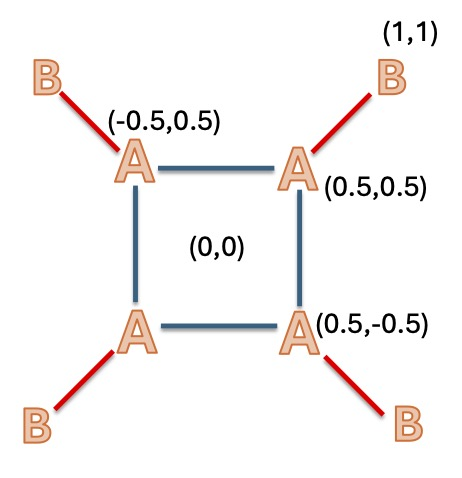
\includegraphics[width=0.5\linewidth]{figures/squareVecBody.jpg}
    \caption{A fictitious example of a rigid body. The text shows different ways that this can be converted to a vector rigid body. }
    \label{fig:vecRB}
\end{figure}
Note that in this fictitious molecular fragment, I have placed all atoms in the x-y plane and the A atoms have coordinates $(\pm0.5,\pm0.5,0)$ and the B atoms have coordinates  $(\pm1,\pm1,0)$. If we create the rigid body with one translation, then the rigid body coordinates are given by this equation:
$$
\begin{bmatrix}
\vec{r}_1 \\
\vec{r}_2 \\
\vdots \\
\vec{r}_8
\end{bmatrix}
= 
t_1
\begin{bmatrix}
0.5&0.5&0 \\
-0.5&0.5&0 \\
-0.5&-0.5&0 \\
0.5&-0.5&0 \\
1&1&0 \\
-1&1&0 \\
-1&-1&0 \\
1&-1&0 \\
\end{bmatrix}
$$
where the A atoms are the first four atoms. Note that the A-A bond distance will be $t_1$  (in \AA) and the A-B bond distance will be $t_1/\sqrt2$  (in \AA).

We could also partition the A and B coordinates into separate matrices, as is done in this equation:
$$
\begin{bmatrix}
\vec{r}_1 \\
\vec{r}_2 \\
\vdots \\
\vec{r}_8
\end{bmatrix}
= 
t_1
\begin{bmatrix}
0.5&0.5&0 \\
-0.5&0.5&0 \\
-0.5&-0.5&0 \\
0.5&-0.5&0 \\
0&0&0 \\
0&0&0 \\
0&0&0 \\
0&0&0 \\
\end{bmatrix}
+
t_2
\begin{bmatrix}
0&0&0 \\
0&0&0 \\
0&0&0 \\
0&0&0 \\
1&1&0 \\
-1&1&0 \\
-1&-1&0 \\
1&-1&0 \\
\end{bmatrix}
$$
where we have completely separated the A atom and B atom matrices. 

There is another way to formulate this same rigid body that, while completely equivalent to the previous, I think is more elegant and illustrates how vector rigid bodies can be very effectively formulated. In this equation: 
$$
\begin{bmatrix}
\vec{r}_1 \\
\vec{r}_2 \\
\vdots \\
\vec{r}_8
\end{bmatrix}
= 
t_1
\begin{bmatrix}
0.5&0.5&0 \\
-0.5&0.5&0 \\
-0.5&-0.5&0 \\
0.5&-0.5&0 \\
0.5&0.5&0 \\
-0.5&0.5&0 \\
-0.5&-0.5&0 \\
0.5&-0.5&0 \\
\end{bmatrix}
+
t_2
\begin{bmatrix}
0&0&0 \\
0&0&0 \\
0&0&0 \\
0&0&0 \\
0.5&0.5&0 \\
-0.5&0.5&0 \\
-0.5&-0.5&0 \\
0.5&-0.5&0 \\
\end{bmatrix}
$$
the $t_2$ translation now specifies the offset of the B atoms from the A positions, as the coordinates for the first A atom are $(\frac{t_1}{2}, \frac{t_1}{2},0)$ and the  coordinates for the first B atom are $(\frac{t_1}{2}+\frac{t_2}{2}, \frac{t_1}{2}+\frac{t_2}{2},0)$. The A-A bond distance remains as $t_1$ (in \AA) but the A-B bond distance is now $t_2/\sqrt2$ (also in \AA) so this version of the rigid body allows the two bond distances to be independent refineable parameters. The previous version allows that as well, but the meaning of the translations is not as obvious. 

\subsection{Inputting a Vector RB to GSAS-II}
I am not aware of any software that will help with creating a vector rigid body, should you wish to use an idealized geometry -- which is what I recommend. This would seem to require work with trigonometry, paper and pencil to create the input matrix/matrices. However, if you have atomic coordinates and wish to create a single-translation model, in the ``Rigid bodies'' data tree entry, select the ``Vector rigid bodies'' tab and then use the ``Edit Vector Body''/``Extract from file'' menu command. This command read coordinates in a variety of formats. It is described further below in \S\ref{ref:ExtractRB}. However, be sure that the coordinates that you are using are very close to the ideal geometry you want. You do not want to force your model to have inaccuracies from a poorly-chosen CIF. The comments below in \S\ref{idealizedXYZ} on obtaining idealized coordinates may also be of value. 

If you have created the coordinate matrices, you can input them using the ``Edit Vector Body''/``Add rigid body'' menu command. This will open a window asking how many atoms are in the body and how many translations will be needed. The data window will then have input fields where you can specify the coordinates, translations and atom type for each row in the first matrix, as seen in Fig. \ref{fig:vecRBinp}. 
\begin{figure}
    \centering
    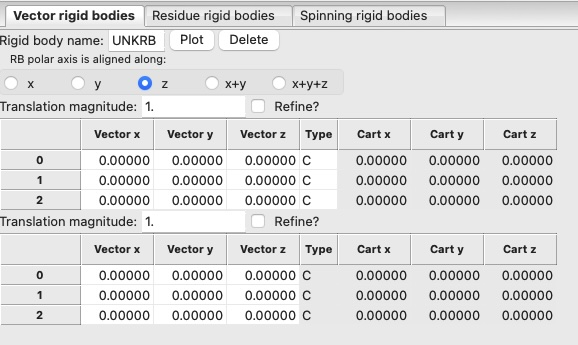
\includegraphics[width=0.5\linewidth]{figures/vecRBinp.jpg}
    \caption{Vector rigid body input window}
    \label{fig:vecRBinp}
\end{figure}
If you would prefer to create input in a text editor, you can create template file by creating a body with the correct number of atoms and translations and then use the ``Edit Vector Body''/``Save rigid body'' menu command to create a \texttt{.vecbody} file, which can then be edited and read in using the ``Edit Vector Body''/``Read rigid body'' menu command.

\section{Residue Rigid Bodies}\index{rigid body!residue|textbf} 
The original GSAS program only offered vector rigid bodies, but GSAS-II also allows a seconf type of rigid bodies to be defined. This type is called a residue rigid body and they have several advantages. The name comes from macromolecular crystallography because the part of an amino acid that remains in a protein after peptide synthesis is called a residue in biochemistry. The residue rigid body implementation was initially for amino-acid residues for proteins, but has considerable utility for organic and organometallic materials as well. While the residue rigid body does not offer refineable translation parameters, it does allow for defining refineable torsion angle parameters. 

\begin{figure}
    \centering
    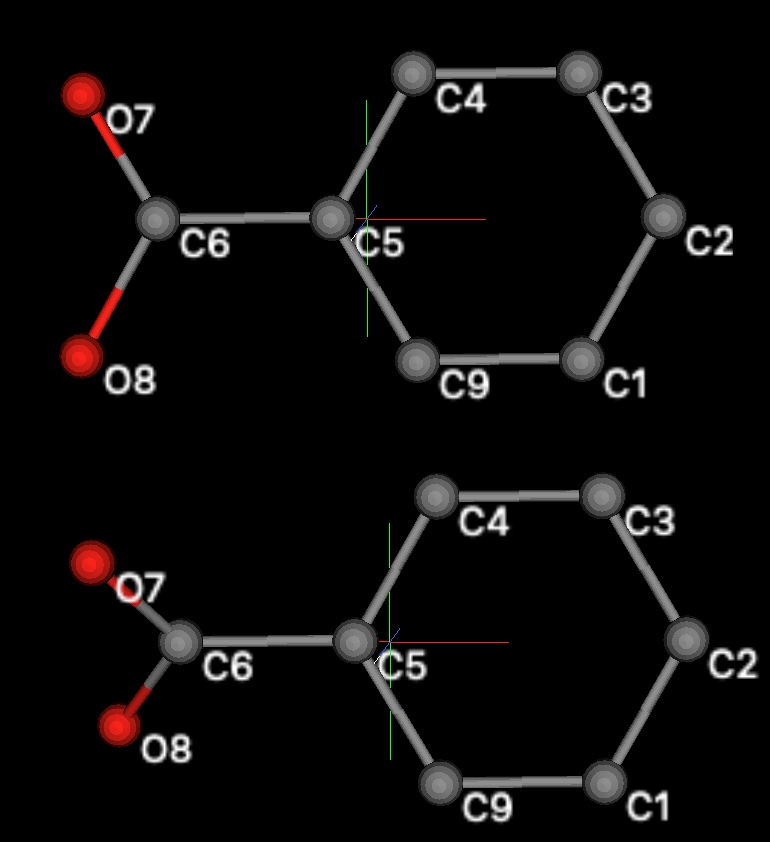
\includegraphics[width=0.5\linewidth]{figures/resRBtorsion.jpg}
    \caption{Visualization of a torsion rotation. The C5-C6 bond has been designated as the torsion and the bond has been rotated by $45^\circ$ between the upper and lower depictions.}
    \label{fig:resRBrot}
\end{figure}

The process for defining a residue rigid body is more straightforward than the fairly complex process of defining a vector rigid body. You will simply supply Cartesian coordinates (in \AA) for the atoms in the rigid body. Should you wish to add torsional degrees of freedom, you do this by designating the pairs of atoms that have the bond between them. Of those two atoms, one is called the ``torsion origin'' and the other ``the pivot.'' The atoms bonded to the pivot atom (called the riding atoms) and the atoms bonded to those atoms, and so on, are the ones that will be rotated as the torsion angle is changed. However, GSAS-II does not include H (or D) atoms as riding atoms. If H atoms are part of the group of atoms attached via a torsion, their position should be generated in the phase's Atoms tab using the ``Edit Atoms''/``On selected atoms...''/``Calc H atoms'' and the ``Edit Atoms''/``Update H atoms'' menu commands. 
A visual example of a torsion rotation is shown in Fig. \ref{fig:resRBrot}. Here the C5 atom is the origin atom for the torsion and the C6 atom is the pivot, so that the riding atoms are O7 and O8. Since there are no H atoms attached to the phenyl ring, had the origin and pivot been switched, the ring would have rotate and the O atoms would stay in their original position. These two approaches are equivalent. Use of either definition for the torsion origin and riding atoms would result in a refinement with differing rigid body parameters, but the resulting crystallographic structures should be the same, within a fraction of the s.u. values. 


\begin{figure}
    \centering
    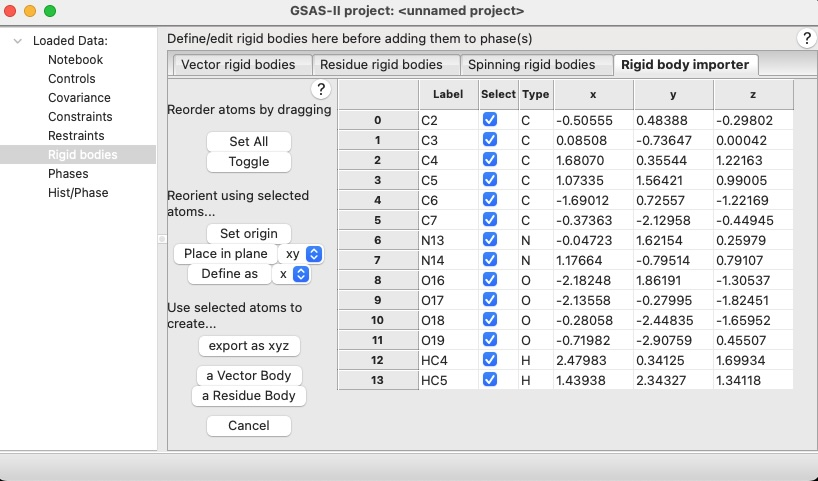
\includegraphics[width=0.75\linewidth]{figures/RBimport.jpg}
    \caption{Creating a rigid body: window created by ``Extract from File'' menu command}
    \label{fig:RBcreate}
\end{figure}
\subsection{Inputting a Residue RB to GSAS-II}
To define a residue rigid body, select the ``Rigid bodies'' data tree entry and then click on the ``Residue rigid bodies'' tab and then use one of the commands in the ``Edit Vector Body'' menu. The menu command choices include:

\subparagraph{``Import XYZ''} This command will read Cartesian coordinates, for example from Avogadro or MolDraw, and will place the atoms into a residue rigid body. 

\subparagraph{``Extract from file''}\label{ref:ExtractRB} This opens a new tab labeled ``Rigid body importer'' where a multistep process is implemented for reading fractional coordinates and selecting atoms to be included. 
\begin{enumerate}
    \item Before attempting to use crystallographic coordinates to create a rigid body, confirm that the atoms you will want to use are all in the same asymmetric unit\index{asymmetric unit}. You may need to reorganize which symmetry replicants are present and possibly even need to lower symmetry. 
    \item In the first step after you press on the ``Extract from file'' menu command, you identify a file to read from. This uses the phase importers (see \S\ref{ref:PhaseImporter} for more information on importers), so any of the formats that GSAS-II supports can be used. 
    \item Once the file is opened and read, you select the atoms that you want to use for creating the rigid body. The atoms in the asymmetric unit are displayed in the graphics window, with unselected atoms made much darker than selected atoms. Press ``Continue'' when you have selected the desired atoms. 
    \item The next window is shown as Fig. \ref{fig:RBcreate} and is quite sophisticated. The atoms that have been included from the previous step are now shown as a ball-and-stick model in the graphics window, where atoms are labeled with their number and element type.  The upper two buttons on the left are used to select atoms, or selection can be done individually in the table. 
    \item The middle three buttons are used to align the origin and axes. This is discussed in more detail below in \S\ref{ref:resRBaxes}.
    \item The there bottom buttons (which will create a vector body, a residue body or cancel the import) will complete this import operation and close the ``Rigid body importer'' tab. The ``export as xyz'' will write a file but does not close the tab. Note that only the selected atoms will be used. This means that atoms can be selected from structure file in step 3, that can be used for defining axes in step 5, but will not be included in the final rigid body if they are not selected in this step.
\end{enumerate}

\subparagraph{``Define torsion''} This is used to add a torsion to a residue rigid body. You will be asked for the two atoms that define the bond. You can add as many torsion angles as is appropriate for your rigid body. The value of the angle torsion angle is an increment that is added to the initial torsion angle from the input Cartesian coordinates. The angle is measured clockwise looking from the rider atoms towards the torsion's origin atom. 
\subparagraph{``Import residues''} This command provides access to macros useful for working with proteins, but is unlikely to be used in any other context. 
\subparagraph{``Save/Read rigid body''}
The ``Save rigid body'' menu command writes the rigid body information to a file named with the extension \texttt{.resbody} and the ``Read rigid body'' will read them back. This is useful to duplicate a rigid body in a separate GSAS-II project. 
\begin{figure}
    \centering
    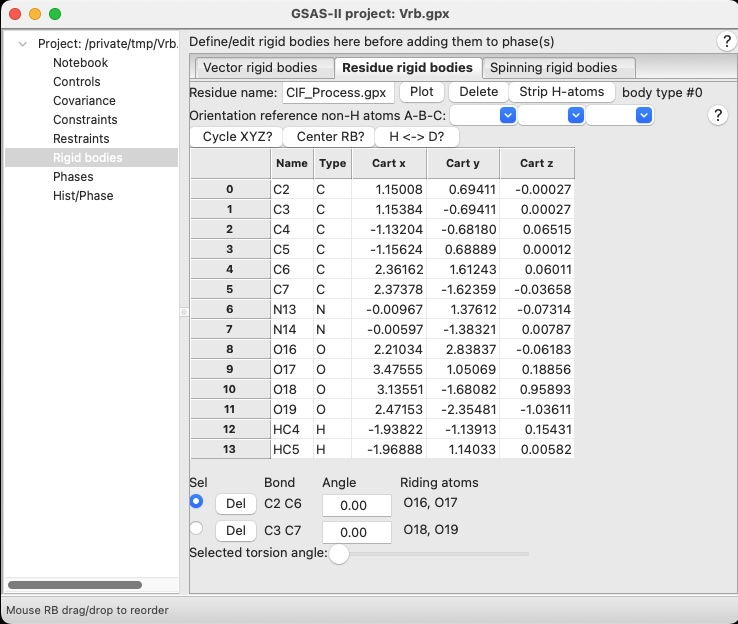
\includegraphics[width=0.75\linewidth]{figures/resRBmain.jpg}
    \caption{The residue rigid body data window. This is seen after a residue rigid body has been created.}
    \label{fig:resRBmain}
\end{figure}

When the residue rigid body is read into the GUI, the data window will appear as in Fig. \ref{fig:resRBmain}. Here, torsions have also been defined. At this stage, only very minimal editing is possible. The orientation of the axes and the origin can be changed here by specifying three atoms for the ``Orientation reference'' settings, which are labeled as A, B and C. The first atom (A) will be set as the origin and the vector from the A atom to the second atom (B) will define the x-axis. The third atom (C) will define the y-axis so that the A, B and C atoms all lie in the x-y plane. The origin for the axes can optionally be changed using the ``Center RB'' button, which will set the origin to center of the rigid body (determined by averaging all coordinates \textit{without} weighting for mass). The use of this will be demonstrated in \S\ref{ref:createPZDC}. Note that if the ``Orientation reference'' settings are changed after use of the ``Center RB'' button, the origin is reset to the ``A'' atom. 

The other controls on this window are: The name for the rigid body is set in the ``Residue name'' box. (It will be made unique if a name is repeated.) The ``Plot'' button displays the rigid body as a ball-and-stick diagram, where atoms are labeled by the atom name. The ``Delete'' buttton will delete this rigid body.  The ``Strip H-atoms'' button is only present if the rigid body contains hydrogen atoms and will remove all H or D atoms from the body. The ``H<->D'' button will replace all H atoms with D ($\rm^2H$)  or the reverse, if pressed again. The ``Cycle XYZ'' button permutes the x, y and z axes. 

\section{Rigid Body Axes and Origin}
Note that when we discuss rigid bodies, we have two independent coordinate systems. One for the rigid body, which does not have any translational symmetry and where the coordinate system is Cartesian; the axes are orthogonal and the coordinate units are in \AA. The crystal system, where translational symmetry is present, uses fractional coordinates and the angles between axes are dictated by the crystal system as we have seen throughout the book. There are two steps in using rigid bodies in GSAS-II. In the first step, the body is defined. For this the source information may be in Cartesian or fractional coordinates, but the rigid body information will be stored as Cartesian. In the second step, the atoms in the phase are related to the atoms in the rigid body. I usually refer to that process as inserting the rigid body into the phase. In that second step, we will determine how the rigid body coordinate system is transformed to produce atom positions in fractional coordinates via position and orientation parameters for the rigid body. Also note that if a rigid body appears in multiple places in a phase (or even several phases in a project), it only needs to be defined once and can be inserted as many times as is needed. Each insertion will have separate position and orientation parameters.

\subsection{Selection of Rigid Body Axes and Origin}
In many cases, it does not matter how the Cartesian axes for the rigid body are oriented with respect to the atoms. However, as will be discussed in detail in \S\ref{ref:RBsym}, if the rigid body will lie on a symmetry axis, plane or point in the unit cell, that axis or plane must be aligned with the Cartesian axes, so that that it can be oriented with respect to the crystal axes. The best location for the origin of the rigid body is at the center of mass for a body, particularly if TLS refinement will be used (discussed in \S\ref{ref:RBTLS}), but if the rigid body will be located on a special position point (most commonly this will be a $\overline{1}$ operator), the origin of the rigid body \textit{must} preserve that symmetry. Even when a rigid body will be placed in a location of the unit cell without any special symmetry, it is still a good idea to define the rigid body axes and origin in a way that represents any symmetry of the fragment. For example, if many of the atoms in the rigid body lie on a plane, I will try to align the axes so that those atoms have one coordinate as approximately zero; usually, I will put those atoms into the x-y plane. 

\subsubsection{Use of the ``Extract from file'' menu command}\label{ref:resRBaxes}
If the coordinates are imported from a file, the axes and origin can be determined from computations in the window created in the second step after use of the ``Extract from file'' menu command (seen in Fig. \ref{fig:RBcreate}). There are three actions that can be performed here: 
\begin{enumerate}
    \item \textbf{Set origin}: To use this, select one or more atoms from the table. If a single atom is selected then the origin is shifted to the location of that atom, so its coordinates will be (0,0,0); if multiple atoms are selected, the origin is shifted to the site midway between the selected atoms. This is not a true center-of-mass as the averaging is not mass-weighted. After selecting atom(s), press the ``Set origin'' button to perform this. 
    \item  \textbf{Place in plane}: Note that the plane to be selected can be the xy, the xz, or the yz plane. The axes orientation is shifted so that the selected plane will be placed to minimize the root-mean-square distance to the selected atoms. The origin is not changed. After selecting three or more atoms, and selecting the plane to use, press the ``Place in plane'' button to perform this. 
    \item \textbf{Define as}: This is used to orient the coordinates so that x, y, or z axis (as selected) points in the selected direction. If one atom is selected here, the coordinate system will be rotated so that x (or y or z) will be oriented so that the axis passes from the origin through the selected atom. If multiple atoms are selected, the axis will pass from the origin to the position midway through the selected atoms. After selecting atom(s) and the axis, press the ``Define as'' button to perform this. 
\end{enumerate}
My experience is that these options work best if used in the sequence listed above, meaning that the top button in the set is used first, then the middle and then the lower button in that order. Note that the atom selection must be repeated yet again, after use of these buttons, to select the atoms in this window that will be included in the vector or residue rigid body. 
\subsubsection{Vector rigid bodies}
For vector rigid bodies, when the coordinates are generated with paper, pencil and calculator, the axes and origin choice are part of the design. If the coordinates are imported from a file, the axes and origin can be determined from settings the window generated by the ``Extract from file'' menu command, as described above in \S\ref{ref:resRBaxes}.
\subsubsection{Residue rigid bodies}
If the ``Import XYZ'' menu command is used to read the coordinates for a residue rigid body, the origin and axes that were defined by the program that created those coordinates will be retained, when the coordinates are read. Likewise, the window created in the second step after use of the ``Extract from file'' menu command (seen in Fig. \ref{fig:RBcreate}) can also be used to set the axes and origin for a residue body as part of the process of converting the coordinates to Cartesian space. 

However, as was presented in the discussion of the residue rigid body data window (seen in Fig. \ref{fig:resRBmain}), the axes orientation and origin values can optionally be overridden by controls there. 
The orientation of the axes and the origin can be changed here by specifying three atoms for the ``Orientation reference'' settings, which I will label as A, B and C. 
The first atom (A) will be set as the origin and the vector from the A atom to the second atom (B) will define the x-axis. 
The third atom (C) will define the y-axis so that the A, B and C atoms all lie in the x-y plane. 

\subsection{Obtaining idealized coordinates}\label{idealizedXYZ}
While you can create a rigid body from fractional coordinates found in a crystal structure, for example from a database, be careful doing this. An individual crystal structure may not have a very accurate representation of the expected interatomic distances and angles and any errors in your rigid body input will be replicated in your results. For this reason, with organic molecular fragments, it is often a good idea to use a molecular forcefield program (unless you have access/ability to use higher-level theory) to obtain an optimized model for the molecule or molecular fragment you wish to use for your rigid body. There are many commercial molecular modeling programs, but if you need something free, the open source Avogadro program\index{software!avogadro|textbf} is a good choice  (\url{https://sourceforge.net/projects/avogadro}). This is available for Windows, Linux or MacOS, or as source code. Note that the XYZ files produced by Avogadro can be read by GSAS-II. A free account on the MolDraw website\index{software!MolDraw website|textbf} (\url{https://www.moldraw.com}) may also work for you. The MOGUL program\index{software!MOGUL} from the Cambridge Crystallographic Database can be used to find the average geometry of a molecular fragment across many crystal structures. 

It should be noted that the molecular modeling, as well as first-principles codes, will compute the ``in vacuum'' structures for the input atoms, corresponding to an isolated object. However, in a crystal structure, molecules and ions will often change configuration to minimize the energetics of packing interactions. In almost all cases, the changes to these moieties will be due to torsion angle changes. It is well worthwhile to review crystallographic results with the moiety to be used for a rigid body to ensure that the common structural configurations can be achieved once torsional modes are included. 

\section{Defining Residue Rigid Body Examples}

It may help to better understand the process of defining a rigid body by following an exercise, where I define two residue rigid bodies. Later in this chapter I will then place these rigid bodies into a metal-organic framework (MOF) material where the two rigid bodies each coordinate a transition-metal atom. The two moieties to be used here are a pyrazine-2,3-dicarboxylic acid ion and a 4,4'-bipyridine (bipy) molecule. 
\begin{figure}
    \centering
    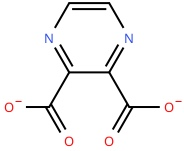
\includegraphics[width=0.25\linewidth]{figures/PyrazinedicarboxylicAcid.jpg}
    \caption{A chemical diagram for the pyrazine-2,3-dicarboxylic acid ion. (Generated with the MolDraw web program.)}
    \label{fig:PZDC}
\end{figure}
\subsection{Create a pyrazinedicarboxylic acid rigid body}\label{ref:createPZDC}
A chemical diagram for the pyrazine-2,3-dicarboxylic acid ion is shown in Fig. \ref{fig:PZDC}. From this we need to obtain a set of three dimensional set of coordinates, which can be done by locating where this molecule has been used in a crystal structure, but my preference is to generate an idealized version of the ion. The two free options for this mentioned earlier in \S\ref{idealizedXYZ} are the Avogadro program or the MolDraw website. In either of these programs, we can ``draw'' the chemical diagram to generate the chemical representation for this, but an easier way to do this is to use the SMILES/indexP{SMILES|textbf} (simplified molecular-input line-entry system) name, which encodes the chemical connectivity. The SMILES notation for the pyrazine-2,3-dicarboxylic acid molecule is readily available from a web search, but the SMILES notation for the deprotonated ion, \mbox{\texttt{C1N=C(C([O-])=O)C(C([O-])=O)=NC=1}}, is likely a bit harder to find. I generated this from the SMILES for the molecule and then deleted the two H atoms. 

If this SMILES string is entered into Avogadro using the Build/Insert/SMILES... the ion will be created. It can then have the geometry optimized using the Extensions/``Optimize Geometry'' menu command, and then the coordinates can be written for GSAS-II using the File/``Save As...'' command (be sure to select the XYZ format). 

While I prefer Avogadro as giving more accurate bond distances and angles, with MolDraw, use their SMILES to 3D Structure Converter (\url{https://www.moldraw.com/tools/free-chem-tools/smiles-to-3d-structure-converter.html}) where you can paste the SMILES entry on the left, click on the ``Render 3D'' button in the middle of the browser window and see the molecule generated in 3D to the right. Click on the ``XYZ'' button in the downloads section under the 3D visual and an \texttt{.xyz} file is downloaded. 

Then we want to create a rigid body with these coordinates in GSAS-II, but there is a minor problem if we want to do this with a new project, because an empty project file does not have any of the overall data tree entries. One must either add a phase or a histogram to the project, and when that is done, the Rigid Body data tree entry will be present. The simplest way to address this is to use the Data/``Add new phase'' menu command to create a phase and then use the Data/``Delete phase entries'' menu command to immediately delete it. However, since you likely have diffraction data to use with the rigid body, you can import that and this will also create the Rigid Body data tree entry. 
\begin{figure}
    \centering
    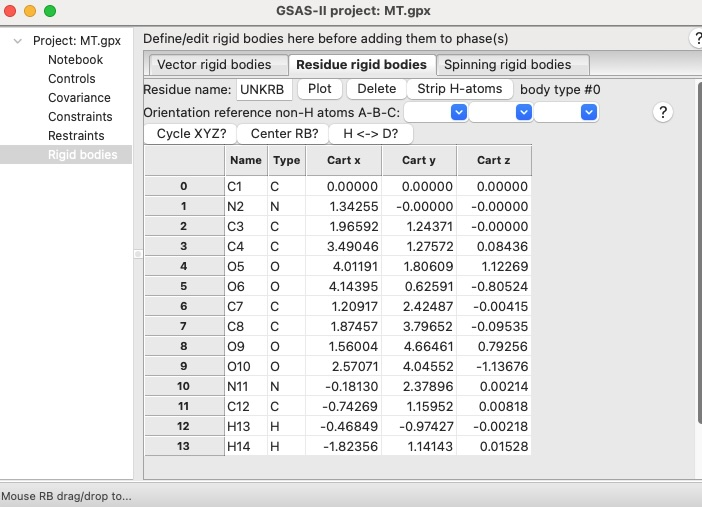
\includegraphics[width=0.7\linewidth]{figures/pzdcRB1.jpg}
    \caption{The Residue Rigid Body data window after reading in the pyrazinedicarboxylic acid XYZ file.}
    \label{fig:pz1}
\end{figure}
To create this rigid body, click on the Rigid Body data tree entry and click on the ``Residue rigid bodies'' tab. Then use the ``Edit Residue Body''/``Import XYZ'' menu command and select the file that was created with Avogadro or MolDraw. The data window will appear as in Fig. \ref{fig:pz1}. Note that this rigid body is not likely to occur in a high-symmetry location in a lattice, as this group of atoms can only have any internal symmetry (one or two mirror planes) when the torsional rotations for the four carboxylate O atoms are matched. Since there is no symmetry present, we do not need to worry about the axes orientations.  Nonetheless, to show how the controls on this data window are used and because I just prefer to have nicely oriented axes, we will select the C1 to C3 vector as the x axis and the C1, C3 and C12 atoms to define the x-y plane, with the y-axis to be in the approximate direction of C1 to C12 by selecting the A-B-C orientation reference atoms to be C1, C3 and C12, as seen in Fig. \ref{fig:pz2}. Press the ``Plot'' button and the ion will be displayed as in  Fig. \ref{fig:pz2p}.
\begin{figure}
    \centering
    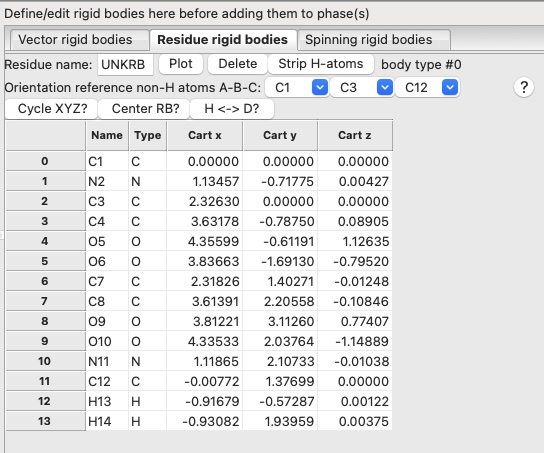
\includegraphics[width=0.5\linewidth]{figures/pzdcRB2.jpg}
    \caption{The Residue Rigid Body data window after setting the orientation atoms for pyrazinedicarboxylic acid.}
    \label{fig:pz2}
\end{figure}
\begin{figure}
    \centering
    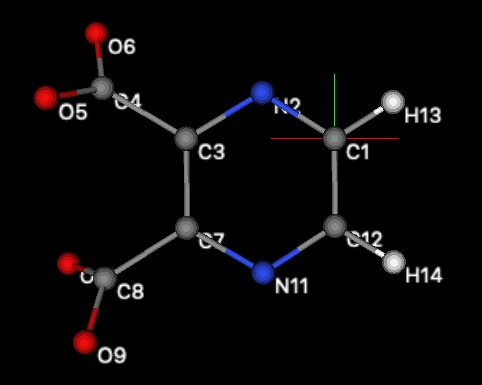
\includegraphics[width=0.4\linewidth]{figures/pzdcRB2p.jpg}
    \caption{The plot of  pyrazinedicarboxylic acid from the Residue Rigid Body data window.}
    \label{fig:pz2p}
\end{figure}
There are still more things that need to be done in this data window. The torsions need to be added to the carboxylate groups, since they depending on the material, they will have very different orientations that optimize bonding. 
This is done by invoking ``Edit Residue Body''/``Define torsion'' menu command. For one torsion angle, use C3 as the origin and C4 as the pivot in the successive input windows. (Note that in the second window the choices are the three atoms bonded to C3.) For the other torsion, use C7 as origin and C8 as pivot. 
You should change the name of the rigid body to something else using the text entry box in the upper left.
While not required, pressing the ``Center RB?'' button will place the origin at a location close to the center of mass. This is useful, as this will simplify TLS fitting (see \S\ref{ref:RBTLS}), should we choose to do that later. After these actions, the ion will be displayed as in  Fig. \ref{fig:pz3p} in the graphics window, where the view point has been moved. The data window appears as seen in Fig. \ref{fig:pz3}. If you will use this rigid body in other GSAS-II projects, you are recommended to save it into a file. This is done with the ``Edit Residue Body''/``Save rigid body'' menu command, which writes a file with extension \texttt{.resbody}. That file can be read in to a different project using the ``Edit Residue Body''/``Read rigid body'' menu command.
\begin{figure}
    \centering
    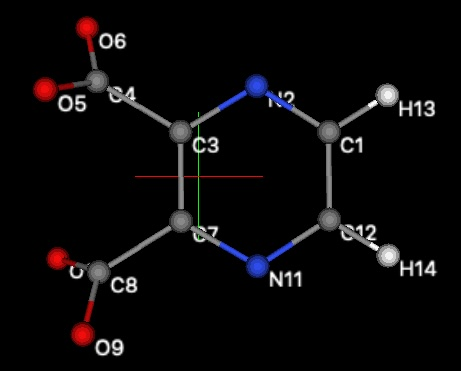
\includegraphics[width=0.4\linewidth]{figures/pzdcRB3p.jpg}
    \caption{The plot of  pyrazinedicarboxylic acid from the Residue Rigid Body data window after the origin has been reset. Note the changed location of the red-green-blue axes location that we call the ``view point'' relative to Fig. \ref{fig:pz2p}. (The blue line is not visible as it is perpendicular to the screen.)}
    \label{fig:pz3p}
\end{figure}
\begin{figure}
    \centering
    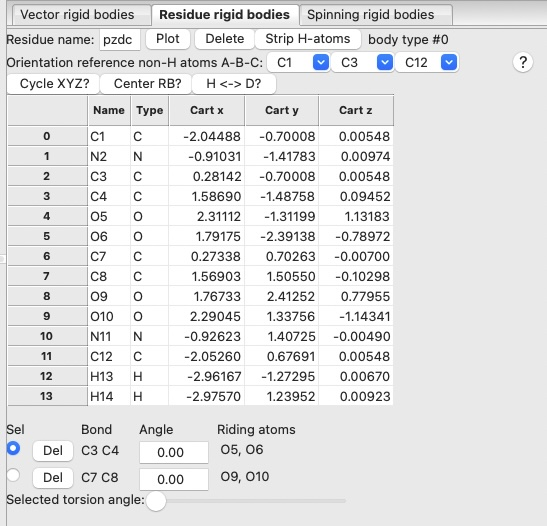
\includegraphics[width=0.5\linewidth]{figures/pzdcRB3.jpg}
    \caption{The Residue Rigid Body data window for pyrazinedicarboxylic acid after setting the origin and rigid body name.}
    \label{fig:pz3}
\end{figure}

\FloatBarrier

\begin{figure}
    \centering
    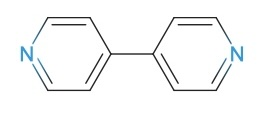
\includegraphics[width=0.25\linewidth]{figures/bipy.jpg}
    \caption{A chemical diagram for the 4,4'-bipyridine molecule. (Generated with the MolDraw web program.)}
    \label{fig:bipy}
\end{figure}
\subsection{Create a bipyridine rigid body}
A chemical diagram for the 4,4'-bipyridine (bipy) molecule is shown in Fig. \ref{fig:bipy}. As before, we need to obtain a set of three dimensional set of coordinates, and again this can be done using the Avogadro program or the MolDraw website. The SMILES notation for the 4,4'-bipyridine molecule is readily available from a web search, \mbox{\texttt{C1=CN=CC=C1C2=CC=NC=C2}}. The same process is used as before in either Avogadro or MolDraw, or any other forcefield or quantum-mechanical modeling program. Interestingly, the Avogadro program creates a planar molecule, while MolDraw provides a molecule with a significant torsion rotation on the bond between the two pyridine groups. Either is fine for our purposes. 

Unlike the pyrazinedicarboxylic acid ion in the previous section, the bipy molecule will always have an internal center of symmetry, regardless of the torsion angle setting. In fact, we will need to place this internal center of symmetry at a specific location in a structure later in this chapter. For this example, we will create two slightly different versions of the bipy molecule that will be used later in the chapter to demonstrate aspects of how GSAS-II handles internal symmetry when rigid bodies are incorporated into the structure. In one case, the rigid body will contain only one-half of the molecule. \textit{e.g.} the unique atoms, and in the other case, we will include both C atoms on either side to the center of symmetry so that the rigid body contains a redundant atom. There is a third option, where we include all the C and N atoms in both rings, but then we would need to delete the H atoms from the torsional riding atom C and that gets a bit more complex than is needed. 

Since we will want to place the origin in a location between two atoms, the ``Import XYZ'' menu command that was used prior will not work for us here. We will instead use the ``Edit Residue Body''/``Extract from file'' menu command which offers more control over the origin and axes location. 

\subsubsection{Half-molecule Bipy}\label{Half-moleculeBipy}
When the ``Edit Residue Body''/``Extract from file'' menu command is used, the first window that is opened asks for the format of the file to be read. In this case, we will read an XYZ file created above, so XYZ is selected. In the next window, select the \texttt{.xyz} file written previously. The contents of the data  window will display the atoms read from the file, as seen in Fig. \ref{fig:bipy0} and the graphics window contents are seen in Fig. \ref{fig:bipy0p}. This visualization will be very useful as we now need to select only the atoms we need for the next step. Unselect atoms 7 through 11 (C7-C10, N2) and 16-19 (H5-H8), leaving only one phenyl ring and the first carbon of the second ring, as seen in Fig. \ref{fig:bipy0p}. Once the atoms are selected, press the ``Continue'' button at the bottom of the data window. 

\begin{figure}
    \centering
    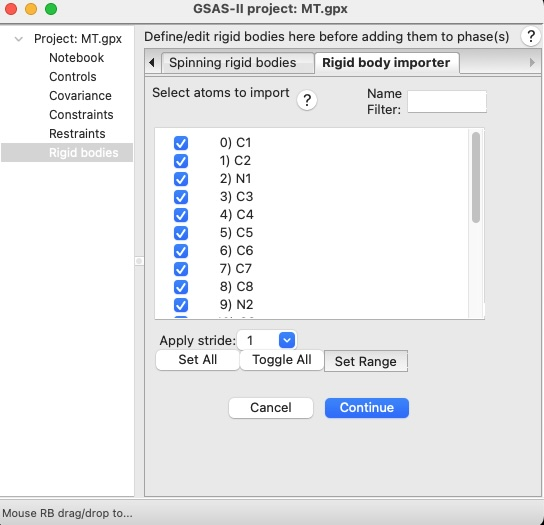
\includegraphics[width=0.65\linewidth]{figures/bipy0.jpg}
    \caption{The initial data window contents when importing the XYZ coordinates for the bipyridine molecule.}
    \label{fig:bipy0}
\end{figure}

\begin{figure}
    \centering
    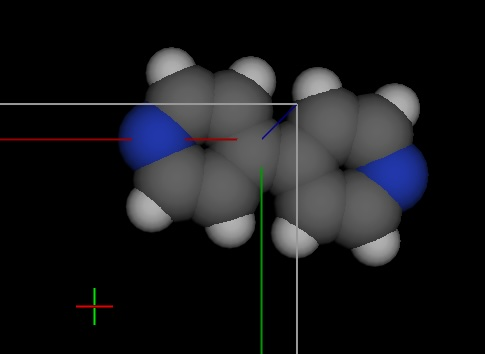
\includegraphics[width=0.45\linewidth]{figures/bipy0p.jpg}
    \caption{The graphics window display when initially importing the XYZ coordinates for the bipyridine molecule. Note that I have used the mouse wheel to enlarge the view of the molecule.}
    \label{fig:bipy0p}
\end{figure}

\begin{figure}
    \centering
    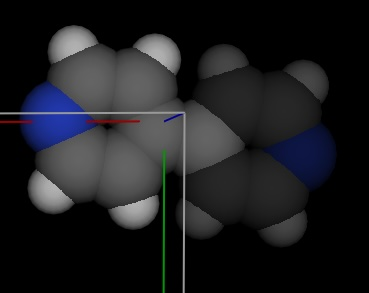
\includegraphics[width=0.4\linewidth]{figures/bipy0pa.jpg}
    \caption{The graphics window display when initially importing the XYZ coordinates for the bipyridine molecule after selection of atoms. The selected atoms appear brighter than the unselected atoms.}
    \label{fig:bipy0pa}
\end{figure}

\FloatBarrier

The data window is then updated, as seen in Fig. \ref{fig:bipy1} and the graphics window contents are seen in Fig. \ref{fig:bipy1p}. This where we have the ability to determine the origin and axes, as was discussed in \S\ref{ref:resRBaxes}. 


\begin{figure}
    \centering
    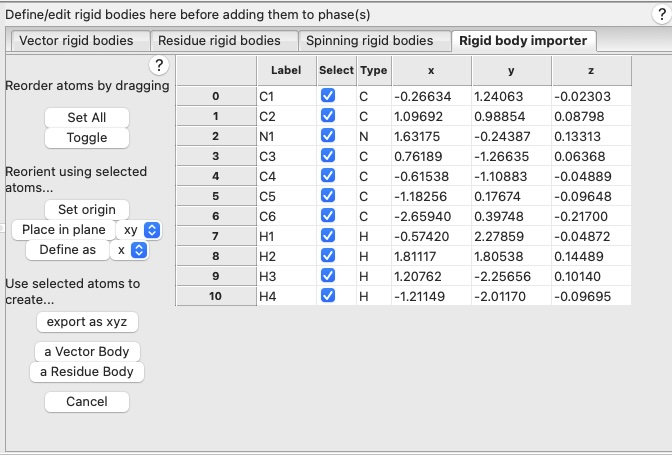
\includegraphics[width=0.75\linewidth]{figures/bipy1.jpg}
    \caption{The second data window contents when importing the XYZ coordinates for the bipyridine molecule.}
    \label{fig:bipy1}
\end{figure}

\begin{figure}
    \centering
    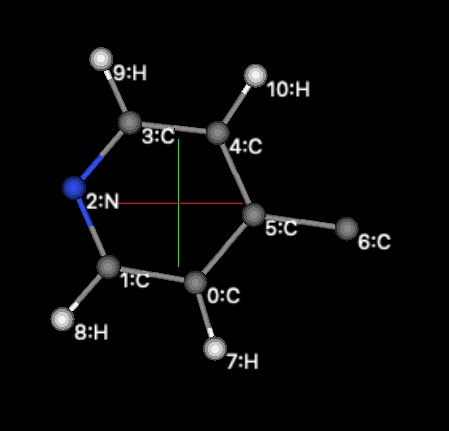
\includegraphics[width=0.45\linewidth]{figures/bipy1p.jpg}
    \caption{The graphics window display after atom selection is complete in the process of defining a bipyridine rigid body.}
    \label{fig:bipy1p}
\end{figure}
Here we want to place the origin midway between atoms 5 and 6 (C5 and C6), so press the ``Toggle'' button, so that no atoms are selected, and then select C5 and C6, and finally press the ``Set origin'' button. Note that the coordinates for these two atoms now add to zero. While for this use, setting the axes is optional, the body will be easier to understand if we place the atoms in one ring into the x-y plane. Select all atoms using the ``Set All'' button and then press the ``Place in plane'' button with ``xy'' selected. Note that z is very close to 0. for all of the selected atoms, confirming that they all do lie in a plane. Finally, we will want to place the x-axis along the C5-C6 bond, so now select either one of those two atoms (but not both as their average position is the same as the origin). Press ``Set All'', then ``Toggle'' and select C5, and finally press the ``Set origin'' button. Note that C5, C6 and N1 now lie on the x-axis as both y and z are now approximately 0. 

Finally, to create the rigid body, we want to remove the one duplicate atom (C6) from the body, so we will want to select all the atoms but that to create the rigid body. Again press ``Set All'' and then unselect the C6 atom. The graphics window will now show the molecule as shown in Fig. \ref{fig:bipy1pF}. To create the  body press the [... create] ``a Residue Body'' button and the second residue body is created. The data window then appears as was seen in Fig. \ref{fig:resRBmain}, except a new control at the top of the window allows you to select between the two rigid bodies that have now been entered. The body will be initially named for the XYZ file, but rename this to ``half-bipy''.

\begin{figure}
    \centering
    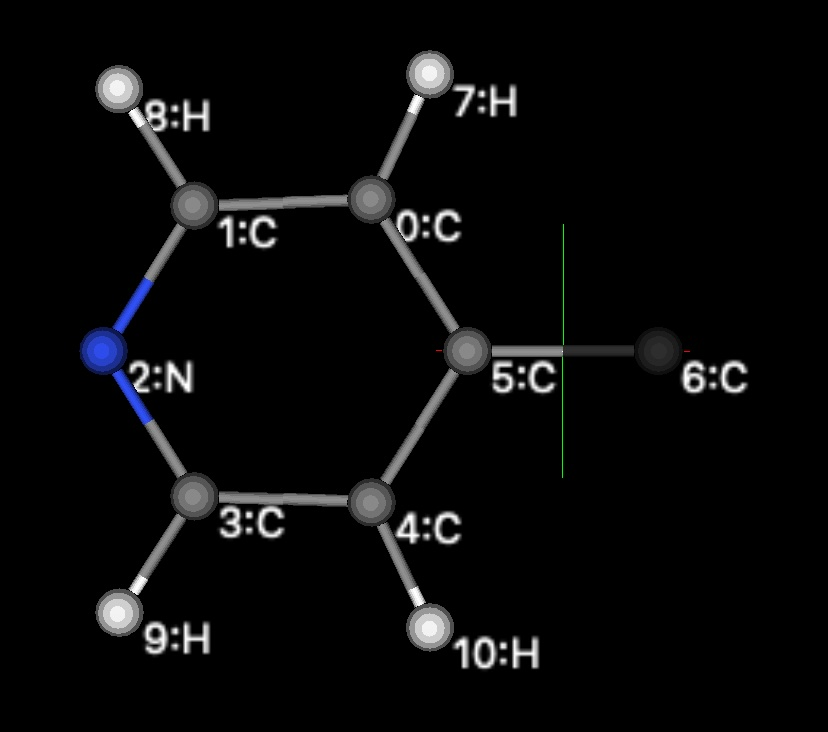
\includegraphics[width=0.45\linewidth]{figures/bipy1pF.jpg}
    \caption{The graphics window display after atom selection is complete in the process of defining a bipyridine rigid body.}
    \label{fig:bipy1pF}
\end{figure}

\subsubsection{Half-molecule+1 Bipy}
To illustrate how GSAS-II handles ``duplicate'' atoms, lets create a rigid body that has both C5 and C6, even though the two atoms will be related by symmetry once the body is inserted into the structure. For this follow the instructions from the previous Half-molecule Bipy section (\S\ref{Half-moleculeBipy}), except that in the final paragraph when we create the rigid body, we want to retain all atoms in the body, including C6) , so we will want to select all the atoms. Again press ``Set All.'' The graphics window will now be similar to Fig. \ref{fig:bipy1pF}, but all atoms will be selected. To create the  body press the [... create] ``a Residue Body'' button and the third residue body is created. Again the data window then appears as was seen in Fig. \ref{fig:resRBmain}, except a new control at the top of the window allows you to select between the three rigid bodies that have now been created. The body will be initially named for the XYZ file, but rename this to ``half-bipy+1''.

\section{Inserting Rigid Bodies}\label{ref:RBinsert}
The process for using rigid bodies in a refinement is a two-step process. First, the rigid body must be defined, as has already been discussed in this chapter. The definition process is independent of any specific crystallographic information on how the body is used and indeed saving the rigid body to a file will allow your hard work to be ``recycled'' in a future project. The second step, which we call inserting the body into a structure, is where the rigid body is integrated into a crystal structure model. (This is what is shown in table in the Atoms tab.) Rigid bodies are added and changed using the ``RB Models'' tab for the phase and are inserted using the ``Edit Body''/``Locate \& Insert Rigid Body'' menu command. Once a rigid body has been selected to insert into the structure, the data window shows information about the rigid body, as seen in Fig. \ref{fig:RBI0} and the insertion process is started. In the insertion process, one defines:
\begin{itemize}
    \item the location of the rigid body origin in fractional coordinates, 
    \item the orientation of the rigid body (see \S\ref{ref:RBquat}),
    \item how the rigid body atoms are mapped to atoms in the structure.
\end{itemize}
\begin{figure}
    \centering
    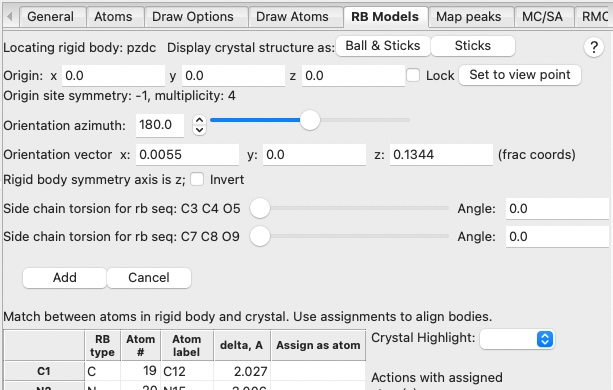
\includegraphics[width=0.5\linewidth]{figures/RBI0.jpg}
    \caption{The data window provided to insert a rigid body. This appears after a rigid body has been selected, but has not yet been inserted.}
    \label{fig:RBI0}
\end{figure}

This process for inserting a rigid body offers several mechanisms to change the position and orientation of the rigid body. One can type numbers into the GUI, or use the azimuth slider and see immediate changes in the graphics window. The mouse can also be used to change the position of the rigid body. Note that the following  mouse actions are defined for the visualization of the structure (discussed in Chapter  \ref{Chap:structureplotting}): 
\begin{itemize}
    \item \textbf{Horizontal Left mouse drag}: left-right mouse movement rotates the structure around the vertical screen axis (y). 
    \item \textbf{Vertical Left mouse drag}: up-down mouse motion rotates the structure around the horizontal screen axis (x). 
    \item \textbf{Right mouse drag}: moves the view point. Since the view point is always at the center of the window, this translates the structure.
    \item     \textbf{Middle mouse drag}: rotates the structure around the screen axis perpendicular to the window (z)
    \item \textbf{Mouse wheel rotation}: this changes the ``camera distance'' which has the effect of zooming the plot in and out.
\end{itemize}
When the Alt key (Option key for MacOS) is held down while using the mouse, the mouse actions reposition the rigid body rather than change the view of the structure:
\begin{itemize}
    \item \textbf{Alt+Left mouse drag}: left-right movement rotates the rigid body around the vertical screen axis (y); up-down motion rotates the rigid body round the horizontal axis (x). The rotation is around the rigid body origin.
    \item \textbf{Alt+Right mouse drag}: Translates the rigid body origin. The motion is in the plane of the window. To move the rigid body in the third direction, rotate the view by $90^\circ$ (using a horizontal left-mouse drag) and then use Alt+right mouse drag. 
    \item     \textbf{Alt+Middle mouse drag}: rotates the rigid body around the screen axis perpendicular to the window (z).
\end{itemize}
Note that with Mac and a single button mouse, it is possible to hold down control+option and use the mouse drag to simulate the right mouse button drag or use command+option to simulate the middle mouse button drag. I recommend getting a three-button mouse, instead. 

The other mechanism for repositioning a rigid body involves specifying pairs of atoms between the rigid body and the structure. The rigid body can be translated and/or oriented so that the specific atoms are moved as close as is possible. This is done with the lower section of the data window, as seen in Fig. \ref{fig:RBI1}. This part of the window is also used to determine how atoms in the rigid body are mapped to atoms in the structure.  I will call the table of atoms shown here as the ``Assignments Table.'' Note that the first two columns of the table show the rigid body label and the atom type. The third, fourth and fifth columns show the atom in the structure that is paired to the rigid body atom, as an atom number, atom label and the distance between the paired atoms. By default, atoms are paired by shortest distances. Note that as the rigid body is moved, these distances are updated and pairing assignments are revised if the closest atoms change. The last column allows one to override this pairing by assigning a specific atom in the structure to be paired to the rigid body atom. 
These assignments are also used for the ``Set Origin,'' ``Set Orientation,'' and ``Set both'' buttons, which will be explained in a subsequent paragraph. 
Optionally, use the ``Update Assignments'' button to the right of the assignments table, after making an assignment to update the list of paired atoms and their distances. 

When the rigid body import process is completed using the ``Add'' button (immediately above the table), the rigid body atom will be added to the phase with the position, orientation, and any torsion angle(s) that has been specified. Each atom in the rigid body will be linked to an atom in the structure where the coordinates, occupancy, and $\rm U_{iso}$ or $\rm U_{\it ij}$ values in the Atoms table will be updated to match what is generated from the rigid body. 
Note that one option for the atom assignments is ``Create new,'' which is used to indicate that a new atom atom should be added to the structure to pair to the rigid body rather than use an atom that is already defined. 

When atom pairs are assigned manually, the ``Set Origin,'' ``Set Orientation,'' and ``Set both'' buttons to the right of the table can be used to set the rigid body location and orientation. At least one atom must be selected for ``Set Origin'' to function. This will set the Origin fractional coordinates to minimize the distance(s) to the paired atom(s). 
If two or more atom pairs are assigned manually, the ``Set Orientation'' button can be used. This sets the Orientation azimuth and Orientation vector values to minimize distances. With three or more atoms assigned, the ``Set both'' button will set the Orientation azimuth and vector as well as the origin coordinates. The use of these will be illustrated later (in \S\ref{ref:RBinsertExample}).

One potentially tricky aspect of assigning atom pairs manually is determining which atoms should be paired. This can be aided by highlighting atoms in the graphics window. If you select a row in this lower section of the data window by clicking on the rigid body label, that atom in the rigid body is highlighted by changing its color to green. Likewise, the paired atom in the structure is also highlighted by changing that atom's color to green. Should you wish to find a different atom in the structure, the ``Crystal Highlight'' selection to the right of the assignments table can be used to select an atom to highlight. 
\begin{figure}
    \centering
    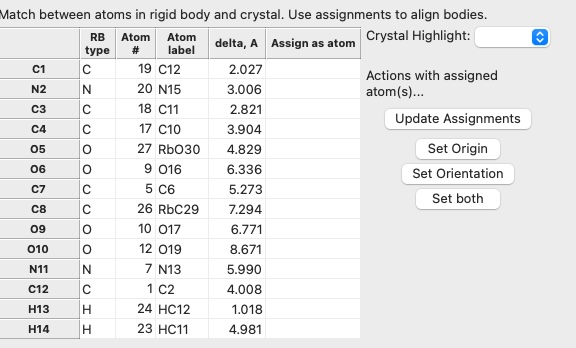
\includegraphics[width=0.5\linewidth]{figures/RBI1.jpg}
    \caption{Enter Caption}
    \label{fig:RBI1}
\end{figure}

Once the body has been inserted, a window such as what is seen in Fig, \ref{fig:RBmodel1}. Note that this window shows the location of the rigid body origin in fractional coordinates, the azimuthal angle and a unit vector in fractional coordinates that position and orient the body. There are refinement flags for the origin and orientation. The refinement modes for orientation refinement (A, V, and AV, which are explained in the next section.) This window allows the overall fractional occupancy for the rigid body to be refined. As noted before, if the Alt key is held down (the Option key for MacOS), the rigid body is moved or rotated rather than changing the view of the entire model. 

There are a number of ways that the ADPs for rigid bodies can be fit. The default is where all atoms are assigned the same $\rm U_{iso}$ value but Translation-Libration-Screw (TLS) group motion descriptions (see \S\ref{ref:RBTLS}) are also offered. 
\begin{figure}
    \centering
    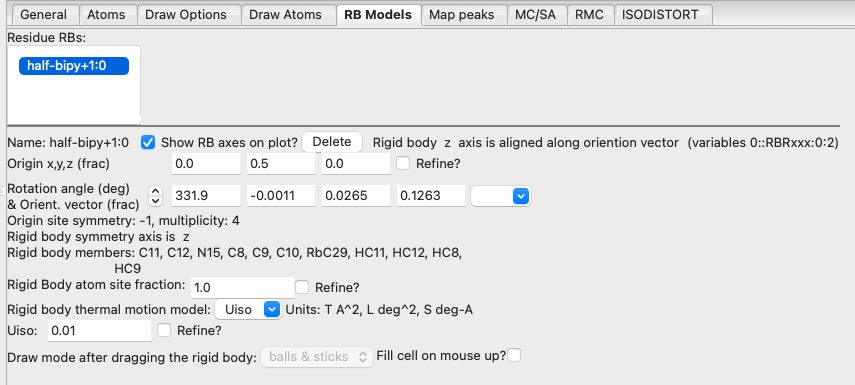
\includegraphics[width=0.8\linewidth]{figures/RBmodel1.jpg}
    \caption{The data window after a rigid body has been inserted into a structure.}
    \label{fig:RBmodel1}
\end{figure}
\section{Orienting Rigid Bodies: Quaternions}\label{ref:RBquat}
When a rigid body is placed into a crystal structure, one must define where in the structure the body will be placed and also how the Cartesian axes of the body will be defined relative to the crystal axes. Understanding how to locate the rigid body is straightforward. That position (in fractional coordinates) is referred to as the rigid body origin, since this is the location of the rigid body's Cartesian coordinate system origin. The mechanism used to orient the rigid body Cartesian axes with the crystal axes is a bit more complex, as will be discussed next.

There are two commonly used mathematical methods for orienting objects, Euler angles\index{Euler angles} and quaternions\index{quaternions}. Quaternions are newer, dating back only to the mid-1800's, in contrast to Euler's work in the mid-1700's. Quaternions are significantly preferable for computational use, but this was not discovered until the past few decades and probably due to needs for video game programming. (GSAS used Euler angles for rigid bodies.) I have read somewhere that ``a quaternion is simply a scalar and a vector combined together into a complex number.'' I'd question the use of ``simply'' in that sentence, but the basic idea is that quaternions use four numbers $q_0$, $q_1$, $q_2$ and $q_3$ but these are normalized so that  $\sqrt{q_0^2 + q_1^2 + q_2^2 + q_3^2} = 1$, so that in fact only three of the four values are unique. 

As was seen in the previous section, instead of displaying the quaternion values, they are converted to a related form, with a unit vector and an azimuthal rotation angle. This unit vector is usually shown in fractional coordinates. This is done in most places where GSAS-II uses quaternions. The math for the conversion is pretty simple, and can be seen in routine \texttt{GSASIImath.Q2AV()}, with the angle in radians, and \texttt{GSASIImath.Q2AVdeg()}, in degrees. The inverse operations are in \texttt{GSASIImath.AV2Q()} (radians) and \texttt{GSASIImath.AVdeg2Q()} (degrees). When GSAS-II refines quaternions, it does so with two refinement flags, one for the vector part of the quaternion and one for the azimuthal angle. Thus, there are four modes for refinement of the orientation quaternion:
\begin{enumerate}
    \item \textbf{AV mode}: In this mode, all of the three degrees of freedom are refined. The name is chosen to indicate that both the azimuth and the vector are fit. 
    \item \textbf{V mode}: In this mode, only two degrees of freedom are refined. The name is chosen to indicate that only the vector is fit. 
    \item \textbf{A mode}: In this mode, only one degree of freedom, that of the azimuthal rotation,  is refined. The name is chosen to indicate that only the azimuth is fit. 
    \item \textbf{None}: In this mode, there are no orientational degrees of freedom.
\end{enumerate}
Symmetry will determine which of these modes is allowed, as will be discussed in the next section. 

\section{Rigid Bodies and Crystallographic Symmetry}\label{ref:RBsym}
It is fairly common that a rigid body will have internal symmetry, such as the 6/m symmetry of the C atoms in a phenyl group; it is somewhat less common for the crystal symmetry to enforce some or all of the symmetry of the rigid body. When this does occur, the rigid body must be placed at a special location (a point, axis or plane) where that crystallographic symmetry is present. As will be discussed here, placement of the rigid body and its refinement will require special attention, but that will require that the rigid body coordinates be defined to be compatible with that symmetry and that the rigid body then be incorporated into the unit cell axes in a manner that preserves the symmetry. The rigid body definition must align the Cartesian axes and/or origin to the internal symmetry in the body: 
\begin{itemize}
    \item If there is a rigid body symmetry axis, it must be defined in Cartesian space along x, y or z (or x+y or x+y+z). Use of x, y, or z is recommended as it is much simpler. 
    \item The Cartesian origin must be defined to match symmetry points or planes in the body
\end{itemize}

The following sections of this chapter will discuss details for how the the rigid body is inserted into the unit cell. However, before we get to that, let's consider how symmetry affects this process. 

\begin{itemize}
    \item The rigid body must be inserted into the crystal structure to place the quaternion rotation vector along the selected Cartesian axis. This is computed for you by GSAS-II. 
    \item The location for the rigid body (the origin), in fractional coordinates, will be a higher-symmetry Wyckoff site rather than a general position.
    \item The rigid body in fractional coordinates origin in crystal space must be constrained to stay on the axis or plane or point of that Wyckoff site and it will not be possible to refine all six degrees of freedom for the rigid body. The site symmetry will determine what parameters can be refined, as will be considered for the different possible symmetry cases, below.
\end{itemize}

When a rigid body is placed at a general position in fractional coordinates, the x,y \& z coordinates for the rigid body positions are all refined, but symmetry may require a constraint such as x=0 or x=y. Note that when individual atoms occur on a high-symmetry site, GSAS-II will generate the constraints that force the atom to remain on that symmetry location, but for rigid bodies, these constraints must be generated manually. These are created using the Constraints data tree entry where you can place a ``Hold'' (see \S\ref{ref:Hold}) on the parameters that should not change. This requires knowing the names for the rigid body location parameters, which are determined from two numbers that are assigned to each rigid body in a project and in a structure. Each rigid body that is created in a project is assigned a number. These numbers start at 0; the number is shown on the data window for vector and residue rigid body, as seen in the example in Fig. \ref{fig:pz3}. In addition, each rigid body can be used multiple times within a phase. These are also numbered and are known as the insertion number. 
The parameter names for residue bodies locations are \texttt{RBRPx:}\textit{n}\texttt{:}\textit{m}, \texttt{RBRPy:}\textit{n}\texttt{:}\textit{m}, and \texttt{RBRPz:}\textit{n}\texttt{:}\textit{m} for the x, y \& z fractional coordinates of the rigid body origin, respectively, 
where \textit{n} is the rigid body number and \textit{m} is the insertion number.
For vector bodies parameter names are 
\texttt{RBVPx:}\textit{n}\texttt{:}\textit{m}, \texttt{RBVPy:}\textit{n}\texttt{:}\textit{m}, and \texttt{RBVPz:}\textit{n}\texttt{:}\textit{m},
for the x, y \& z fractional coordinates of the rigid body origin, respectively. 

\subsection{Symmetry Cases}
The possible ways that symmetry can interact with rigid bodies follows:

\subparagraph{Center of symmetry} The Cartesian origin will need to be the $\overline{1}$ position, so the rigid body origin will need to be placed at the site of symmetry for the rigid body. 
This will always be either on an atom in the group or at the midpoint between two (or, occasionally more) atoms. 
There is a choice here with respect to which atoms will be included. One can include only one from each symmetry-related pair of atoms in the body, or both. If symmetry-related atoms are included, GSAS-II will recognize them and will set the occupancy to zero for one atom of each pair of duplicates. Note that in this case ($\overline{1}$), there are no requirements for the orientation of axes.

In crystal coordinates: when the rigid body is inserted into the structure, the origin location will need to selected as a $\overline{1}$ site in the structure. 
Since that symmetry location is a fixed point in fractional coordinates, no coordinates can be refined. The body orientation can be refined in ``AV'' mode (no orientational constraints).
%No special care for occupancies will be needed as GSAS-II should set these for you. 

\subparagraph{Mirror plane} The rigid body must be defined so that the normal to the mirror plane will be along a fixed Cartesian axis for the body; use of x, y, or z for that axis is recommended. 
The Cartesian origin must be defined so that it lies in the mirror plane. \textit{I.e.}, if z will be the direction normal to the mirror plane, then the rigid body's internal mirror plane must be placed at z=0.

In crystal coordinates: One coordinate in the rigid body origin will need to be fixed on the mirror plane. So that the origin may be refined, you will need to place a constraint hold (see \S\ref{ref:Hold}) on parameter \texttt{RBRPx:}\textit{n}\texttt{:}\textit{m}, \texttt{RBRPy:}\textit{n}\texttt{:}\textit{m}, or \texttt{RBRPz:}\textit{n}\texttt{:}\textit{m}. If located on in a diagonal mirror planes, you will need to place an equivalence between x, y and/or z.   The rigid body orientation vector will need to be fixed along the mirror plane normal, so this can't be refined. Only the rigid body azimuth angle can be refined (mode ``A''). Thus there are three free parameters: two for position and one for orientation.  
%Occupancies: Consider if atoms are duplicated, if so lower frac relative to atoms on the plane

\subparagraph{Rotation axis} The Cartesian origin must be defined on the rigid body's symmetry axis, which will be on an atom or at a midpoint between two or more atoms. Align the rigid body's symmetry axis along a fixed Cartesian axis;  use of x, y, or z for that axis is recommended. 

In crystal coordinates: the coordinates for the rigid body origin will need to be constrained to stay on the axis by placing holds (see \S\ref{ref:Hold})  or constraints on two origin parameters (\texttt{RBRPx:}\textit{n}\texttt{:}\textit{m}, \texttt{RBRPy:}\textit{n}\texttt{:}\textit{m}, and/or \texttt{RBRPz:}\textit{n}\texttt{:}\textit{m}.) The rigid body orientation vector will need to be fixed along the axis in crystal coordinates. For orientation only the rigid body azimuth angle can be refined (mode ``A''). 
Thus there are two free parameters for the body: one for position and one for orientation.  

\subparagraph{Improper rotation axes} define both an axis and a perpendicular plane. It will be uncommon to find a rigid body on an improper rotation axis, but if this occurs, the Cartesian origin must be fixed on the point where the axis meets the plane and a Cartesian axis must be chosen along the symmetry axis for the rigid body. 

In crystal coordinates,  the origin is fixed to be at the point where the axis and plane intersect in fractional coordinates. The rigid body Cartesian axis must be aligned with the crystallographic rotation axis.  The only degree of freedom for refinement will be the rigid body azimuth angle (mode ``A'').

\subparagraph{Glide planes and screw axes} are unlikely to occur with rigid bodies, as the molecular fragment for the body would have to have internal symmetry that includes translational symmetry; the rigid body would need to be part of an infinite-length molecule. I would be very interested to see an example of this. 

\subsection{Linear Rigid Bodies}

A linear rigid body has two orientational degrees of freedom rather than three, since a rotation of the object along the linear axis leaves it unchanged. The linear rigid body will usually be defined so that the linear axis falls on one of the Cartesian axes. (Note exception below for a body in a symmetry plane). 
The specific requirements depend on the symmetry for the location where the inear rigid body will be placed. 

\subparagraph{General position}: when a linear rigid body is placed in a location with no symmetry, there are no restrictions on the origin location or the orientation. The origin can be refined freely and the orientation can be refined in ``V'' mode (with two degrees of freedom) for a total of five refinable parameters. 

\subparagraph{Linear Rigid Body in a Symmetry Plane} 
This provides a minor challenge, in that there can be only one orientational degree of freedom, since rotation along the rigid body linear axis leaves the body invariant and the body must remain in the plane. The solution to this is that the body orientation must be defined so that the azimuthal axis is normal to the plane so that if refined in ``A'' mode, the body rotates in the plane. The origin can be placed anywhere along the body, but is best in the middle. The origin for the rigid body will have two degrees of freedom (use appropriate constraints). 

\subparagraph{Linear Rigid Body Perpendicular to a Symmetry Plane} 
In this case, there are no orientational degrees of freedom. The origin must be placed in the middle of the body, and will have two degrees of freedom so that the body can move in the plane (use appropriate constraints). 

\section{Example: Inserting rigid bodies}\label{ref:RBinsertExample}

For this, we will approximately duplicate the structure model used in the MOF structure from Silvana Urcia-Romero \textit{et al.} (2022), Crystal Growth \& Design, 2382–2391.\footnote{DOI: 10.1021/acs.cgd.1c01460}. The CIFs from this paper can be downloaded for free from the CCDC \footnote{\url{https://www.ccdc.cam.ac.uk/structures/search?pid=ccdc:2125626\&issn=1528-7483\&id=doi:10.1021/acs.cgd.1c01460\&sid=ACS}}. Any of the CIFs from that paper will do. After the coordinates are read, and the ``Draw Atoms'' or ``Draw Options'' phase tab is selected, the structure will appear as shown in \ref{fig:MOF0}.
\begin{figure}
    \centering
    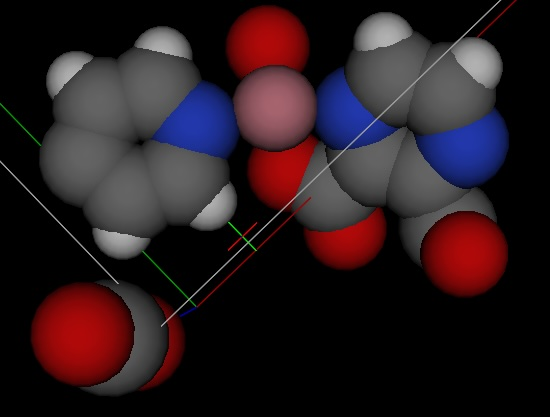
\includegraphics[width=0.5\linewidth]{figures/MOF0.jpg}
    \caption{The asymmetric unit for the MOF structure being used to demonstrate use of rigid bodies. The pink atom is Co, which is bonded to a bipyridine (half shown), a pyrazinedicarboxylic acid unit and a water molecule. Also present is a $\rm CO_2$ molecule. Note that the view point has been shifted away from the center of the unit cell.}
    \label{fig:MOF0}
\end{figure}

\subsection{Example 1: Inserting the pyrazinedicarboxylic acid ion rigid body}

To insert the pyrazinedicarboxylic acid ion rigid body that was previously created, select the ``RB Models'' phase tab. 
If for some reason the structure is not plotted, select the ``Draw Atoms'' or ``Draw Options'' phase tab and then return to the `RB Models'' tab. 
The `RB Models'' tab posts the menu labeled ``Edit Body'' and from that menu select the ``Locate \& Insert Rigid Body'' menu command. This will open a window where one can select from the three rigid bodies that were previously defined. The body we want was called ``pzdc''; select this and press OK. The data window will appear, as seen in Fig. \ref{fig:RBI0} and the structure visualization will appear as shown in \ref{fig:MOF1}, where now the rigid body is also displayed. 

\begin{figure}
    \centering
    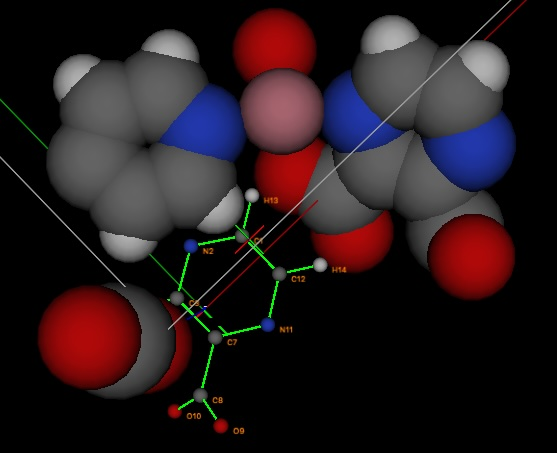
\includegraphics[width=0.5\linewidth]{figures/MOF1.jpg}
    \caption{The asymmetric unit for the MOF structure with the addition of the pyrazinedicarboxylic acid rigid body in the process of being inserted. The stick figure with green lines for bonds shows the rigid body location and orientation.}
    \label{fig:MOF1}
\end{figure}

Our next task will be to orient the pyrazinedicarboxylic acid rigid body on the approximate positions of the atoms that are in that group. This will be very hard to see with these atoms shown as space-filling. Press the ``Ball \& Sticks'' or ``Sticks'' button to change the display according to your preference. As noted before (in \S\ref{ref:RBinsert}) we can identify atoms to be paired by highlighting them. The most easily identified atoms to me are the ring nitrogens and the carboxyilic carbons. In Table \ref{tab:pzatoms} I have provided a list of atoms to be paired. 
\begin{table}
    \centering
    \begin{tabular}{cc}
     rigid body    & structure \\
         N2& N13\\
         N11& N14\\
         C4& C6\\
         C8& C7\\
    \end{tabular}
    \caption{Easily identifiable paired atoms for the pyrazinedicarboxylic acid rigid body and corresponding atoms in the structure.}
    \label{tab:pzatoms}
\end{table}
Assign these four atoms, as seen in Fig. \ref{fig:RBI2}. Then press the ``Set both'' button and note that the rigid body is now largely superimposed, as seen in Fig. \ref{fig:MOF2} and the assignments table (Fig. \ref{fig:RBI3}) now shows the C and N paired atoms are all within a few tenths of an Ångstrom. The O atoms can be brought into better agreement by adjusting the torsion angles with the sliders.  
\begin{figure}
    \centering
    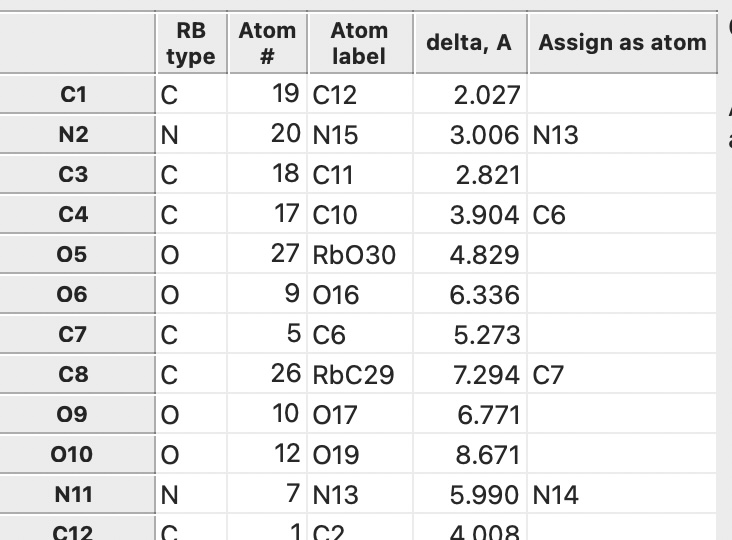
\includegraphics[width=0.35\linewidth]{figures/RBI2.jpg}
    \caption{The assignments table for the pyrazinedicarboxylic acid rigid body, which shows how atoms are paired. This is after four atom assignments have been made, but before the rigid body position has been updated.}
    \label{fig:RBI2}
\end{figure}
\begin{figure}
    \centering
    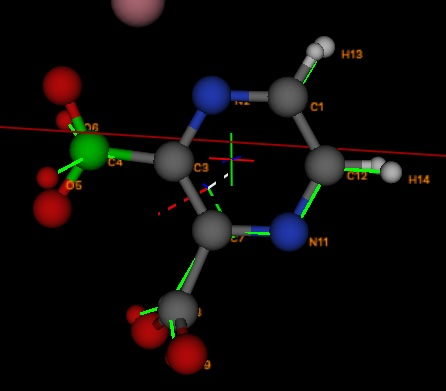
\includegraphics[width=0.5\linewidth]{figures/MOF2.jpg}
    \caption{The pyrazinedicarboxylic acid rigid body superimposed on the structure, in the process of being inserted.}
    \label{fig:MOF2}
\end{figure}
\begin{figure}
    \centering
    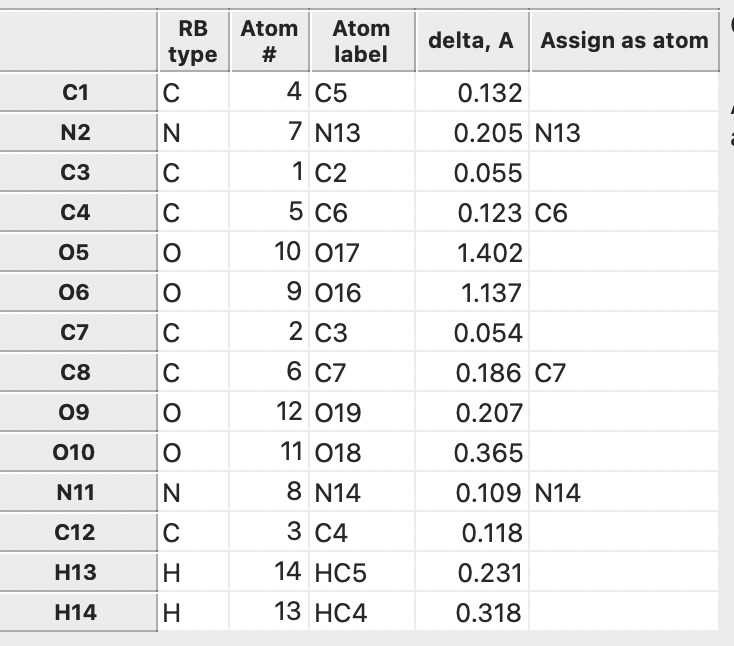
\includegraphics[width=0.35\linewidth]{figures/RBI3.jpg}
    \caption{The assignments table for the pyrazinedicarboxylic acid rigid body after four atom assignments have been made and the ``Set both'' button has been used to superimpose the bodies. Note the close distances between the C and N atom pairs.}
    \label{fig:RBI3}
\end{figure}

Finally, complete the rigid body insertion process by pressing the ``Add'' button. The two sets of superimposed atoms are replaced by a single set, where the bonds are now colored in orange, to indicate that this is a rigid body, as seen in \ref{fig:MOF3}. The positions of the rigid body atoms are updated in the Atoms tab and the coordinates and $\rm U_{iso}$ values are shaded to indicate that these values are generated from the rigid body, as seen in Fig. \ref{fig:RBI4}.
\begin{figure}
    \centering
    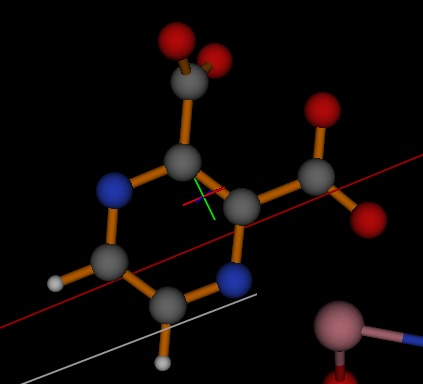
\includegraphics[width=0.5\linewidth]{figures/MOF3.jpg}
    \caption{The pyrazinedicarboxylic acid ion rigid body after insertion. The orange bonds indicate that this is a rigid body.}
        \label{fig:MOF3}
\end{figure}
\begin{figure}
        \centering
        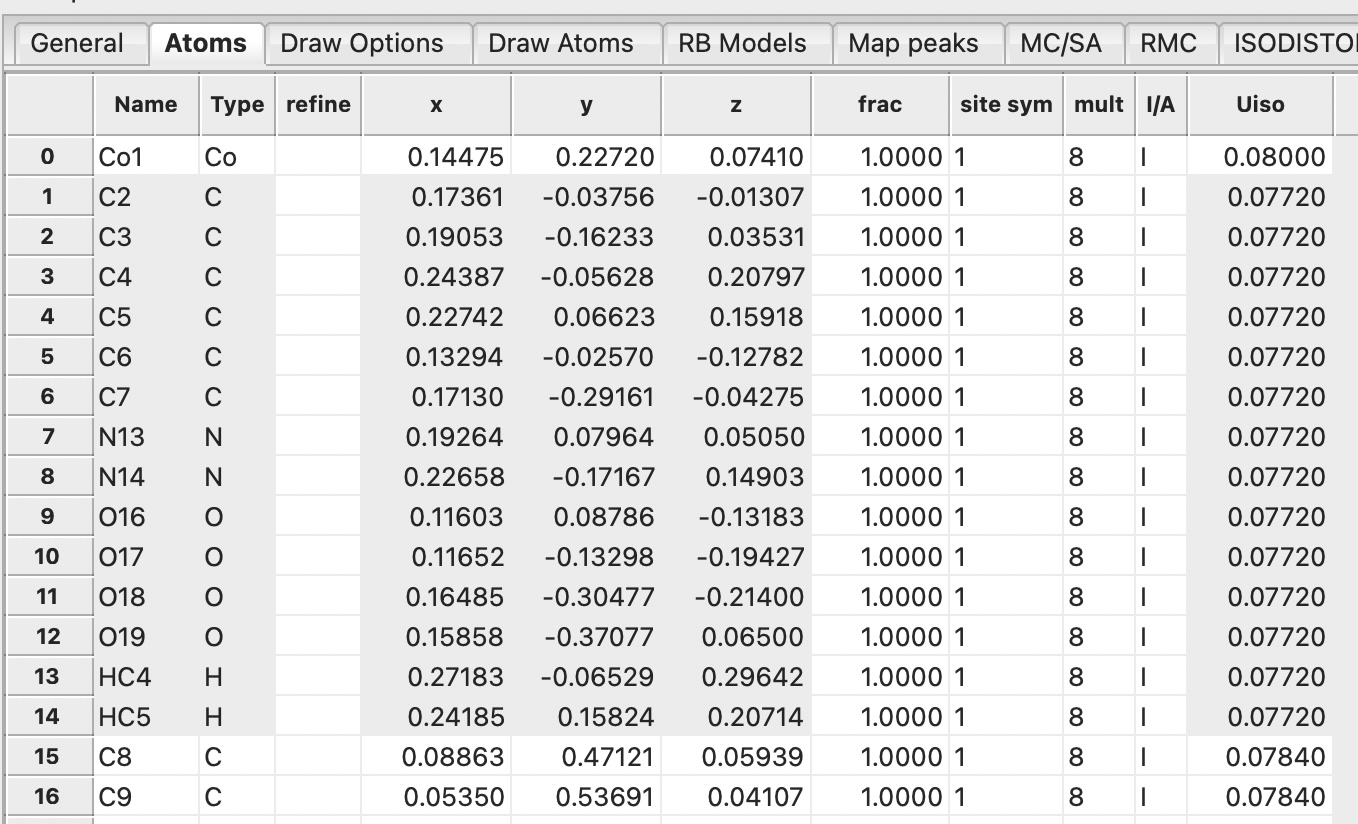
\includegraphics[width=0.5\linewidth]{figures/RBI4.jpg}
            \caption{The contents of the Atoms tab after the pyrazinedicarboxylic acid ion rigid body has been inserted. Note the shading of the coordinates and $\rm U_{iso}$ values to indicate that these values are generated from the rigid body. }
        \label{fig:RBI4}
    \end{figure}
    
\subsection{Example 2A: Inserting the bipyridine molecule rigid body}
Before beginning this example, you should save the GSAS-II project so that we can return to this point, where only the first rigid body has been inserted. 
This rigid body is a bit different from the previous because it has internal symmetry. It is duplicated by a center of symmetry. This $\overline{1}$ located at (0,$\frac{1}{2}$,0), so this is where the origin of this rigid body needs to be placed. 
% would be nice if this worked, but the RB Models tab overrides this:
% The graphics will be a bit easier to use if the view point is placed at this location. Change the ``View Point'' setting on the Draw Options tab to \texttt{0 0.5 0} and so that you see the same plot as I will show, change the ``View Dir.'' setting to \texttt{0 0 1} so that the view is down \textit{c}.

Again, select the ``RB Models'' phase tab, if needed. 
To insert the bipyridine molecule rigid body from the ``half-bipy'' rigid body that was previously created; again use the ``Edit Body''/``Locate \& Insert Rigid Body'' menu command. This will open a window where one can select from the three rigid bodies that were previously defined. The body we want was called ``half-bipy''; select this and press OK. The data window will appear similar to what was seen before (Fig. \ref{fig:RBI0}) and the half-molecule bipyridine rigid body is also displayed. 

 To set the origin location, change the ``Origin'' y value to 0.5 at the top of the data window and select the ``Lock'' selection so this does not get changed accidentally. At this point, given that the origin is fixed, it is not that hard to use the Alt+Left mouse and Alt+Middle mouse drag motions to align the rigid body to the atoms in the structure. This will not be easy to explain in writing how to do this, but let me try. Note that the following paragraph is optional as the following one duplicates the alignment process.

The initial plot appears with the rigid body approximately opposite where we want it, as seen in Fig. \ref{fig:RBI5}. Holding the Alt key down, drag the middle mouse button (Alt+middle mouse) vertically until the two rings are approximately aligned, as seen in Fig. \ref{fig:RBI6}. While this looks to be fairly reasonable alignment, rotating the view by approximately $90^\circ$, by dragging with the left mouse button (no Alt key) produces a view that shows the rings are not in the same plane, as seen in Fig. \ref{fig:RBI7}. Rotation of the rigid body using Alt+left mouse, will bring the rings to be closely overlapped. 
\begin{figure}
    \centering
    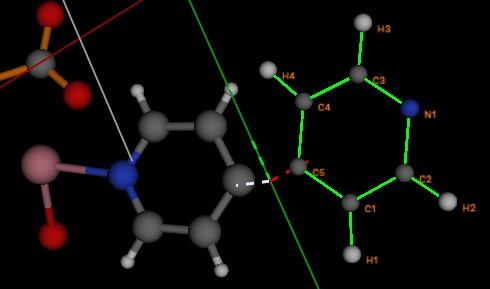
\includegraphics[width=0.5\linewidth]{figures/RBI5.jpg}
    \caption{Initial location of the half-bipyridine molecule rigid body during the insertion process.}
    \label{fig:RBI5}
\end{figure}
\begin{figure}
    \centering
    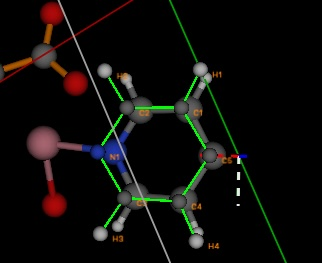
\includegraphics[width=0.45\linewidth]{figures/RBI6.jpg}
    \caption{Location of the half-bipyridine molecule rigid body during the insertion process after rotation using the Alt+middle mouse button.}
    \label{fig:RBI6}
\end{figure}
\begin{figure}
    \centering
    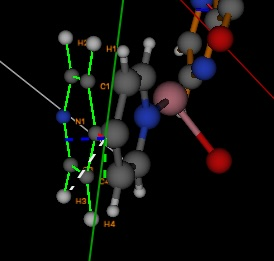
\includegraphics[width=0.4\linewidth]{figures/RBI7.jpg}
    \caption{Location of the half-bipyridine molecule rigid body during the insertion process after rotation using the Alt+middle mouse button and rotation of the view.}
    \label{fig:RBI7}
\end{figure}

The other way to align the rigid bodies is to assign atoms, as was done before.
Note that the rigid body N1 atom must be paired to the N15 atom in the structure. The two rigid body atoms bonded to N1 are C2 and C3, which can be seen from the atom labels in the plot. In the structure, it can be determined that C8 and C12 are bonded to N15 using the ``Crystal Highlight'' option. As before, assign these atoms. Assign rigid body atoms C2, N1, and C3, respectively, to structure atoms C8, N15, and C12, respectively, and press the ``Set Orientation'' button. (Note that it does not matter if C8 is assigned to C2 or to C3, so the two C atoms assignments could be reversed.)

Finally, press ``Add'' to complete the insertion of this rigid body. The half of the bipyridine molecule will now appear with orange bonds, as was seen before for the pyrazinedicarboxylic acid. 

\subsection{Example 2B: Inserting the bipyridine molecule rigid body with a duplicate atom}
The last example will be to repeat the previous rigid body insertion, but to use a version of the rigid body that includes atoms that are duplicated by symmetry. The rigid body insertion in previous step needs to be reversed before this step can be performed. Either reload the GSAS-II project (\texttt{.gpx}) file that was saved in the last step or delete the rigid body insertion by selecting the \texttt{half-bipy:0} body on the ``RB Models'' tab and then press the ``Delete'' button. 

Follow approximately the same process as before to insert the bipyridine molecule rigid body. Again use the ``Edit Body''/``Locate \& Insert Rigid Body'' menu command, but this time use the ``half-bipy+1'' rigid body that was previously created, . This will open a window where one can select from the three rigid bodies that were previously defined. Again, set the origin location by changing the ``Origin'' y value to 0.5 at the top of the data window and select the ``Lock'' selection. Assign rigid body atoms C2, N1, and C3, respectively, to structure atoms C8, N15, and C12, respectively, and press the ``Set Orientation'' button. 

One important extra step is needed relative to the previous example. While atoms C1-C5, N1, and H1-H4 match atoms in the structure, there is no matching atom for C6. The default action would be to pair this atom with one of the $\rm CO_2$ C atoms, but here we need is for GSAS-II to add this atom to the structure when the rigid body is inserted. From the pull-down menu in the ``Assign as atom'' for C6, select the ``Create new'' option. Then press the ``Update Assignments'' button and the assignments table should appear, as in seen in Fig. \ref{fig:RBI8}. 
\begin{figure}
    \centering
    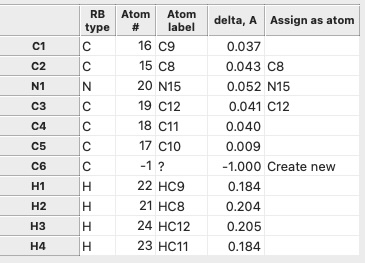
\includegraphics[width=0.35\linewidth]{figures/RBI8.jpg}
    \caption{The assignments table for the bipyridine molecule+1 rigid body. Note that atom C6 has been designated as a new atom.}
    \label{fig:RBI8}
\end{figure}
After the ``Add'' button has been pressed, the rigid body information is updated in the Atoms tab, which appears as in seen in Fig. \ref{fig:RBI9}. Note that the C6 atom in the rigid body has been added to the atoms list as atom \#29 (the second atom labeled as RbC29.) Note that since this atom is a symmetry duplicate, the occupancy has been set as zero during the insertion process. 
\begin{figure}
    \centering
    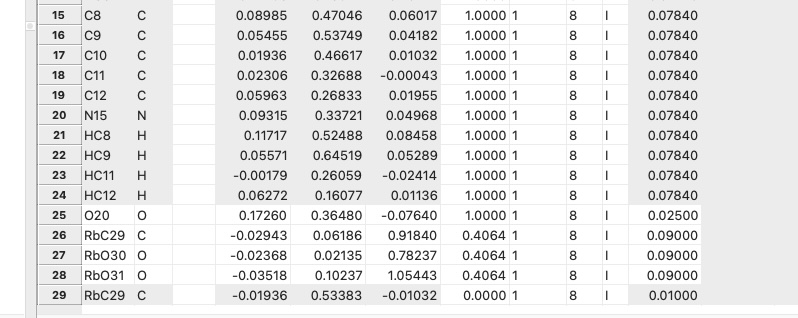
\includegraphics[width=0.75\linewidth]{figures/RBI9.jpg}
    \caption{The contents of the Atoms tab after the bipyridine molecule+1 rigid body has been inserted. The new atom from the rigid body has been inserted as the last atom.}
    \label{fig:RBI9}
\end{figure}
\section{TLS Displacement Parameters for Rigid Bodies}\label{ref:RBTLS}

Translation-Libration-Screw (TLS) representation was initially presented by Verner Schomaker\index{Schomaker, V.} and Ken Trueblood\index{Trueblood, K.} in a seminal 1968 \textit{Acta Cryst.} paper (DOI: 10.1107/S0567740868001718) as a mechanism for understanding the motion of rigid bodies from their ADPs. They expanded the representation developed by D. W. J. Cruickshank\index{Cruickshank, D.} who used two tensors to describe group motion, a six-term tensor for anisotropic translational motion, that is labeled ``T'' (for translations) and another a six-term tensor for anisotropic rotational  motion,  labeled  ``L'' for libration.  Schomaker and Trueblood added a third eight-term ``S'' tensor (named for screw motion, which combines translations and librations.) This is now known as the TLS model. Note that for a body that has an origin placed at the center of the rotary motion, the S terms are all zero, greatly simplfying the full TLS representation from 20 terms to 12. For an isolated body, the center of rotation will be the center of mass, but in a crystal, bonds and Van der Waals interactions make the center of rotation less clear. 

Initially, crystallographers fit individual anisotropic ADP values for each atom in the group and then fit TLS terms to the ADP values to extract information about body's motions. Now when TLS fitting is used, the model is invoked directly and ADP values are generated from the T, L and S terms. 

Note that the effect of the T matrix terms, if asymmetrical, will be to have different motion in different crystallographic directions, but motion of each atom due to the contribution of T will be the same. In contrast, the L matrix terms will have greater impact the farther an atom is from the origin of the body. S terms have both effects. In GSAS-II, when atoms in a rigid body are set as isotropic, the ADP will not show the anisotropy generated by the T, L and S terms, as the $\rm U_{iso}$ value will show an average for all directions, but if the rigid body atoms are set to be anisotropic, the anisotropy will be clear from the $\rm U_{\it ij}$ values. In powder diffraction, one seldom has sufficient data to refine as many as six anisotropic parameters for an atom. However, with rigid bodies, since these values are being generated from the TLS terms, there is no disadvantage to using anisotropic parameters for atoms in a rigid body. 

\subparagraph{Fitting TLS terms.} With powder data, I never try to fit all 20 TLS terms. I will assume that my origin choice is close enough to the center of rotation to leave the S terms as all zero. Even the remaining 12 terms may be too many to refine reliably. I may refine only the diagonal T and L terms (for a total of 6 terms) and have been known to even constrain the diagonal terms to all be the same, so that I have only 2 terms to refine for the entire group, but that still allows me to have a feel if rotation or translation is the primary form of group motion. 